% =================================================
%
% This is the LaTeX file for the Bachelor Thesis of
%
%                		Fabian Reitz
%
%						
%
%	   "Chancen und Risiken einer Migration von
%		Webanwendungen zu nativen Anwendungen"
%					
%			 		  in cooperation with 
%						stadt.werk GmbH
%							  and
%			Duale Hochschule Schleswig-Holstein
%
% =================================================

% ------------------------------
%
% Configuration of the document:
%
% ------------------------------

% Dokumenten-Klasse und Format auf A4 festlegen:
\documentclass[a4paper]{scrartcl}

% Einen Zähler für Paragraphen benutzen:
\addtocounter{tocdepth}{1}

% Einrückung bei Absatzbeginn verhindern:
\setlength{\parindent}{0pt}

% ------------------
%
% Benötigte Packages
%
% ------------------

% Europäisches Buchstaben-Encoding verwenden:
\usepackage[T1]{fontenc}
\usepackage{csquotes}

% Deutsche Rechtschreibung nach aktueller Reform verwenden:
\usepackage[ngerman]{babel}

% Fontspec verwenden:
\usepackage{fontspec}

% Code syntax highlighting:
\usepackage{listings}

% Zeilenabstand verwenden:
\usepackage{setspace}

% Bessere Tabellen
\usepackage{tabularx}
\newcolumntype{Y}{>{\raggedright\arraybackslash}X}

% Abschnitte im Dokument verlinken: 
\usepackage{hyperref}
\hypersetup{
	pdfencoding=auto,
	pdftitle={TITEL},
	pdfsubject={THEMA},
	pdfauthor={Fabian Reitz},
	pdfkeywords={},
   	hidelinks
}

% Befehle zum Festlegen der aktuellen Uhrzeit verwenden:
\usepackage{scrtime}

% Einbinden von Grafiken:
\usepackage{graphicx}
\usepackage{float}
\usepackage{sidecap}

% Include Checkmarks: 
\usepackage{bbding}
\usepackage{pifont}
\newcommand{\xmark}{\ding{55}}

% Setzen der Seitenabstände
\usepackage[a4paper, left=4cm, right=4cm, top=3cm, bottom=1.5cm]{geometry}

% Ein Abkürzungsverzeichnis benutzen:
\usepackage{acronym}

% Den Header des Dokumentes bearbeiten:
\usepackage{fancyhdr}

% Inhaltsverzeichnis und Abbildungsverzeichnis in 
% das Inhaltsverzeichnis einbinden:
\usepackage[notbib]{tocbibind}

% Setzen von Punkten als Trenner in das Inhaltsverzeichnis:
\usepackage[titles]{tocloft}
\renewcommand{\cftsecleader}{\cftdotfill{\cftdotsep}}

% TOC verbessern:
\usepackage{tocloft}

\setlength{\cftbeforesecskip}{3pt}

\usepackage{makecell}

\usepackage{titlesec}

\setcounter{secnumdepth}{4}


\titleformat{\paragraph}
{\normalfont\normalsize\bfseries}{\theparagraph}{1em}{}
\titlespacing*{\paragraph}
{0pt}{3.25ex plus 1ex minus .2ex}{1.5ex plus .2ex}

\usepackage{amsmath}

\usepackage{chngpage}

\usepackage{float}

% Speziell für die Thesis:
% ------------------------

% Biblatex zum Erstellen von Quellenangaben:
\usepackage[
	backend=biber,
	style=ext-authoryear,
	firstinits=true,
	dashed=false,
	maxcitenames=2,
	maxbibnames=99
]{biblatex}

% Bibliography importieren:
\addbibresource{bibliography.bib}

\DeclareNameAlias{sortname}{last-first}
\DeclareFieldFormat{url}{[online]\space\url{#1}}
\DeclareFieldFormat{urldate}{[abgerufen am {#1}]}

\DeclareDelimFormat[bib]{nametitledelim}{\addcolon\space} 

% Den Punkt nach dem Titel durch ein Komma ersetzen:
\usepackage{xpatch}
\xpatchbibdriver{online}
  {\usebibmacro{title}%
   \newunit}
  {\usebibmacro{title}%
   \printunit{\addcomma\space}}
  {}
  {}
% Internet source: Place comma after titleaddon
\renewcommand*{\titleaddonpunct}{\addcomma\space}

% Book source: Place comma after Title
\DeclareFieldFormat[book]{title}{\textit{#1}\addcomma}

% Article source:
\DeclareFieldFormat[article]{title}{#1\addcomma}
\DeclareFieldFormat[article]{journaltitle}{\textit{#1}\addcomma}
\DeclareFieldFormat[article]{volume}{Bd. #1\addcomma\space}
\DeclareFieldFormat[article]{number}{\space Nr. {#1}}
\DeclareFieldFormat[article]{pages}{S. #1 \addcomma}

% Deutsches "u.a." durch "et al." ersetzen:
\DefineBibliographyStrings{ngerman}{
   andothers = {{et\,al\adddot}},
}

% In-Text citing
\renewcommand*{\postnotedelim}{\addcolon\space}
\DeclareFieldFormat{postnote}{#1}
\DeclareFieldFormat{multipostnote}{#1}

% Sources without date
\newcommand{\mkbibnodate}{o\adddot D\adddot}
\AtEveryCitekey{\iffieldundef{year}{\restorefield{labelyear}{\mkbibnodate}}{}}
\AtEveryBibitem{\iffieldundef{year}{\restorefield{labelyear}{\mkbibnodate}}{}}


% --------------------------------
%
% Einstellungen für die Schriftart
%
% --------------------------------

% Schriftart auf "Times New Roman" festlegen:
\setmainfont[
	Path = ./_fonts/,
    BoldFont = Arial-Bold.ttf,
    ItalicFont = Arial-Italic.ttf
]{Arial.ttf}

% Header bearbeiten:
\pagestyle{fancy}
\fancyhf{}
\fancyhead[C]{- \thepage\ -}
\renewcommand{\headrulewidth}{0pt}

\linespread{1.5}



% ---------------------
%
% Anfang des Dokumentes
%
% ---------------------

\begin{document}


% ---------------------
% Deckblatt definieren:
% ---------------------

\begin{minipage}{0.2\textwidth}
	\begin{figure}[H]
		
\includegraphics[scale=0.25]{_assets/logo_DHSH}
	\end{figure}
\end{minipage} \hfill
\begin{minipage}{0.68\textwidth}
	\begin{itemize}
		\item[] \huge BACHELOR-THESIS
		\item[] \large Fachrichtung Wirtschaftsinformatik
	\end{itemize}
\end{minipage} \\


\begin{center}
	\LARGE Chancen und Risiken einer Migration von Webanwendungen zu nativen Systemen 
\end{center}

\begin{tabbing}
	Betreuender Dozent: tabbing \= Mitte \= Rechts \= \kill
	
	\textbf{Studiengruppe:}  			\> 119 WINF \\
	\textbf{Eingereicht von:} 			\> Fabian Reitz \\
										\> Hasseldieksdammer Weg 13 \\
										\> 24114 Kiel \\
										\> +49 175 6392445  \\
										\> fabian.reitz@stud.dhsh.de \\
	\textbf{Erstgutachter DHSH:}			\> Prof. Dr. Alexander Paar \\
										\> Hans-Detlev-Prien-Straße 10 \\
										\> 24106 Kiel \\ 
										\> +49 431 3016255 \\
										\> alexander.paar@dhsh.de \\							
	\textbf{Gutachter des Betriebes:	}	\> Marc Köster \\
										\> Mittelstraße 7 | Hinterhaus \\
										\> 24103 Kiel \\
										\> +49 431 53015400 \\
										\> koester@stadtwerk.org \\
	\textbf{Zweitgutachter DHSH:}		\> Prof. Dr. Michael Sachtler \\
										\> Hans-Detlev-Prien-Straße 10 \\
										\> 24106 Kiel \\ 
										\> +49 431 3016170 \\
	\textbf{Abgabetermin:}				\> 16.05.2022 \\
	
\end{tabbing} 

\thispagestyle{empty}


% -------------------
% Inhaltsverzeichnis:
% -------------------

\newpage

% Alle folgenden Seiten in römischen Zahlen zählen:
\pagenumbering{Roman}

% Beginn der Paginierung bei zwei:
\setcounter{page}{2}

% Inhaltsverzeichnis zeigen:
\tableofcontents


% ----------------------
% Abkürzungsverzeichnis:
% ----------------------

% Neue Seite beginnen:
\newpage

\section*{Abkürzungsverzeichnis}

\addcontentsline{toc}{section}{Abkürzungsverzeichnis}

% Abkürzungsverzeichnis beginnen:
\begin{tabbing}
	----------------------- \= Erklärung \kill
	API \> Application Programming Interface \\
	\> deutsch: Programmierschnittstelle \\
	CP \> Cross-Plattform \\
	\> deutsch: plattformübergreifend \\
	CSS \> Cascading Style Sheets \\
	DOM \> Document Object Model \\
	HTML \> Hypertext Markup Language \\
	IDE \> Integrated Development Environment \\
	\> deutsch: integrierte Entwicklungsumgebung \\
	UI \> User Interface \\
	\> deutsch: Nutzungsoberfläche \\
	W3C \> World Wide Web Consortium \\
	\> deutsch: Internet Konsortium \\
	Webapp \> Web Application \\
	\> deutsch: Webanwendung \\
	WLAN \> Wireless Local Area Network \\
	\> deutsch: drahtloses lokales Netzwerk \\
	
\end{tabbing}


% ----------------------
% Abbildungsverzeichnis:
% ----------------------
\newpage

\listoffigures


% --------------------
% Tabellenverzeichnis:
% --------------------
\newpage

\listoftables

% -----------
% Einleitung:
% -----------

% Neue Seite erstellen:
\newpage

% Paginierung mit eins beginnen:
\setcounter{page}{1}

% Alle folgenden Seiten in arabischen Zahlen zählen:
\pagenumbering{arabic}

% Neue Section: Einleitung
\section{Einführung}

\subsection{Einleitung}
Während es unmöglich ist, den Ursprung des Internets auf einen exakten Zeitpunkt festzulegen, lässt sich jedoch mit Gewissheit sagen, dass die Entwicklung des Internets einen bedeutsamen Wendepunkt in der Geschichte der Menschheit darstellt \autocite[26]{Kleinrock}. \textcite{Floridi} sieht in dem Internet als „Infosphere“ \autocite[9]{Floridi} die vierte Revolution in einer Reihe von weltverändernden Wandlungen. Zu diesen Wandlungen gehören die Kopernikus-Revolution, die Darwin'sche Revolution und die Freud'sche Revolution. Diese Wenden veränderten das grundlegende Verständnis der Menschen sowohl über ihre Umwelt als auch über sich selbst \autocite[8f.]{Floridi}. \\

Das Internet befindet sich in einem stetigen Wandel. Der Beginn des modernen Internets wird im Kontext dieser Arbeit auf den Zeitpunkt datiert, als Sir Tim Berners-Lee die ersten Webkomponenten im Jahr 1990 entwickelte. Berners-Lee arbeitete zu diesem Zeitpunkt bei \textit{CERN} in der Schweiz. Er entwickelte ein System zur Verwaltung von unternehmensinternen Information mittels des ersten Webbrowsers. Dieser war in der Lage, HTML-Dokumente von einem durch Berners-Lee entwickelten Webserver abzurufen und darzustellen \autocite{Berners-Lee}. \\
In der Geschichte des Internets finden sich einige Trends und Entwicklungen, welche als Meilensteine gesehen werden. Diese teilen das Internet historisch in Web 1.0, Web 2.0, Web 3.0 und Web 4.0 auf \autocite[133]{Kollmann}. \\
Den Beginn der Geschichte des Internets bildet das Web 1.0. Dieses basiert überwiegend auf den Ideen von Berners-Lee und wird durch die Etablierung des Internets in der Gesellschaft erweitert. Somit besteht das Web 1.0 lediglich aus statischen HTML-Seiten, welche den Nutzenden in einem Webbrowser angezeigt wird. Der dominierende Webbrowser der Neunzigerjahre ist der \textit{Netscape Navigator} des Unternehmens \textit{Netscape Communications} \autocite{Oreilly}. Besonders für das Web 1.0 ist die binäre Rollenverteilung der Nutzenden, wie Kollmann beschreibt:
\begin{quote}
	„Zum einen gab es aktive Ersteller von Web-Inhalten, die, teils kommerziell, teils privat, Informationen einstellten und publizierten. Zum anderen gab es passive Konsumenten, die sich lediglich die bereitgestellten Inhalte ansehen konnten und auch gar keine andere Option hatten, als die Informationen zu empfangen und zu konsumieren“ \autocite[134]{Kollmann}.
\end{quote}
Dieser Passivität der Konsumierenden sind sich die Unternehmen der Zeit des Web 1.0 ebenfalls bewusst. So zeigen sich im Web 1.0 die ersten Ansätze von ausgefeilten E-Commerce-Strategien, welche darauf abzielen, Produkte und Dienstleistungen auf diesem neuen Markt zu vertreiben \autocite[1204]{Kollmann_Lomberg}. \\
Das auf das Web 1.0 folgende Web 2.0 entstand um 2005 und markierte somit die Zeit, als die dot-com-Blase geplatzt ist. Diese stetige Wende ist aus einer Konferenz zwischen den Unternehmen \textit{O'Reilly} und \textit{MediaLive International}. Die Idee einer nächsten Evolutionsstufe des Internets kam den Unternehmen bei einem Brainstorming. Dieses Brainstorming brachte letztendlich die \textit{Web 2.0 Conference} hervor. Hierbei muss Erwähnung finden, dass Unternehmen das Buzzword \textit{Web 2.0} als Marketing-Element missbrauchen. Das erschwert die Einordnung des Web 2.0 umso mehr, da viele dieser Unternehmen nichts mit den Definitionsansätzen der \textit{Web 2.0 Conference} gemein haben. Die \textit{Web 2.0 Conference} versucht sich an einer Definition über zentrale Aspekte dieser neuen Iterationsstufe des Internets. Dazu gehören die Ansätze \textit{Web as a Platform} und \textit{User-Generated Content}. Die Rolle der passiven Konsumierenden des Web 1.0 veränderte sich demnach zu den aktiven Teilnehmenden des Web 2.0. Erste soziale Medien ermöglichen eine Interaktion mit anderen Nutzenden, Bewertungen auf E-Commerce-Seiten verschaffen Käuferinnen und Käufern eine Stimme und digitale Enzyklopädien laden zum Teilen des eigenen Wissens ein. Zentrale Plattformen des Web 2.0 sind somit \textit{Facebook}, \textit{eBay} und \textit{Wikipedia}. Anbieter einer Rich User Experience, vor allem \textit{Google}, lösen die Riesen des Web 1.0, beispielsweise \textit{Netscape}, ab \autocite{Oreilly}. Dabei spielen die sieben Grundprinzipien des Web 2.0 eine zentrale Rolle: Globale Vernetzung, Kollektive Intelligenz, Datengetriebene Plattformen, Perpetual Beta, Leichtgewichtige Architekturen, Geräteunabhängigkeit und Reichhaltige Oberfläche \autocite[Kollmann und Häsel 2007, zitiert nach][137]{Kollmann}. \\

Die Fortführung, der Ausbau und die allzeitliche Zugänglichkeit des Web 2.0 machen das Internet zu der modernen Infosphere, die Floridi 2010 beschrieb. Durch die Möglichkeiten, die Entwicklerinnen und Entwicklern gegeben werden, ist es mit wenig Aufwand möglich, ganze Anwendungen über einen Webbrowser zugänglich zu machen. Insbesondere Anwendungen, welche ursprünglich für native Systeme entwickelt wurden, finden ihren Weg in die Cloud. Welche Vor- und Nachteile dieser Trend hat und ob eine Remigration zu nativen Systemen unter Verwendung moderner Technologien Sinn ergibt, wird in dieser Arbeit näher beleuchtet. 

\newpage

\subsection{Problemstellung}
Die Entwicklung von Anwendungen für das Web wird eine immer beliebtere Alternative zu nativen Anwendungen, wie beispielsweise installierbare Desktop-Anwendungen. Deutlich erkennbar wird der Trend bei einem Vergleich der \textit{stackoverflow Developer Surveys} aus den Jahren 2015 bis 2021. Betrachtet man nun die Antworten \textit{Full-Stack Developer} und trägt diese als Funktion der Jahre auf, lässt sich folgender Graph erkennen: 

\begin{figure}[H]
	\centering
		\caption{Anteil der Full-Stack Entwicklerinnen und Entwickler von 2013 bis 2021}
	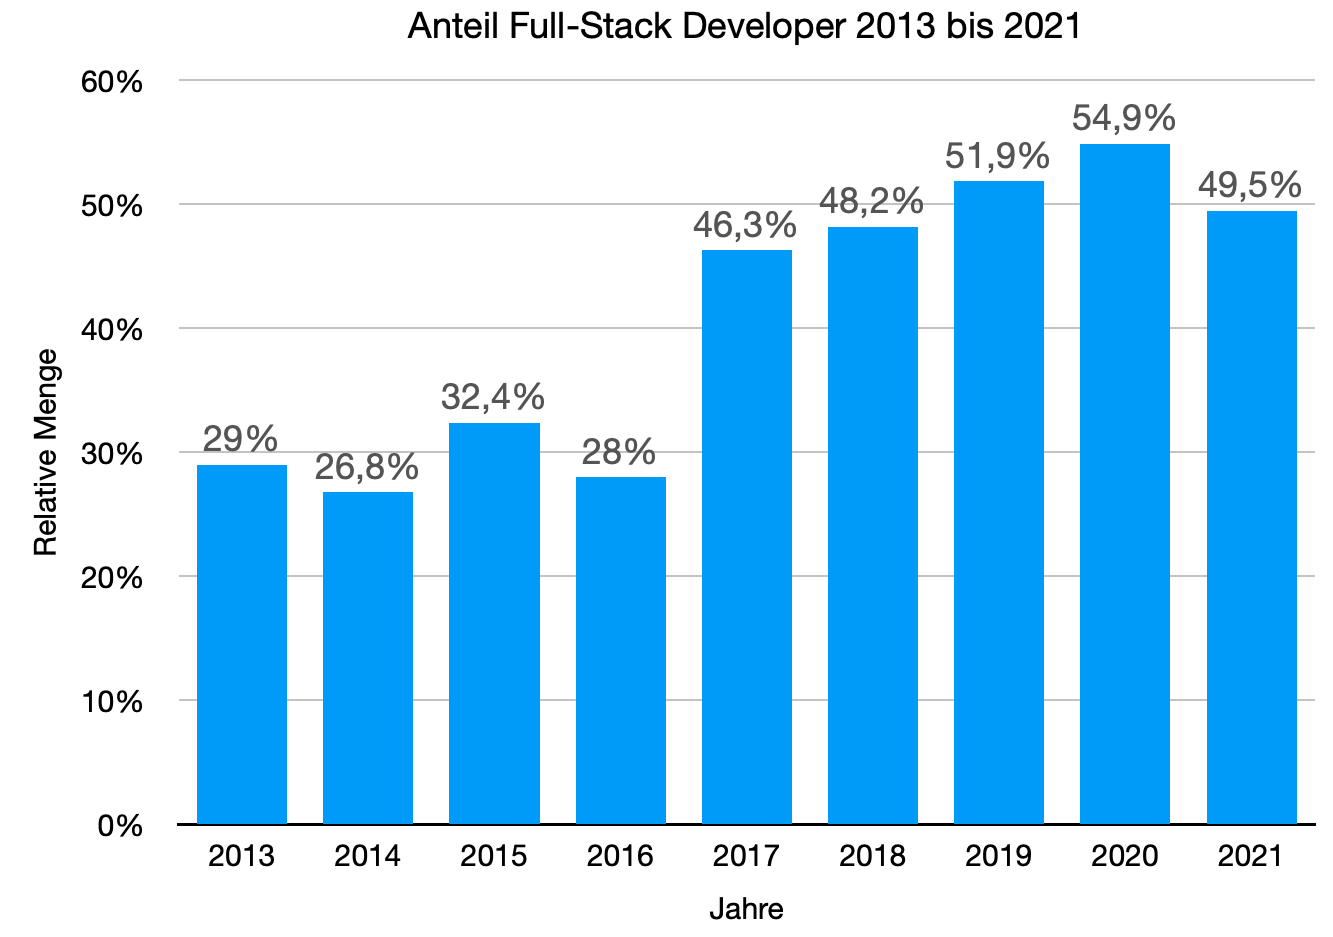
\includegraphics[scale=0.28]{_assets/stackoverflow_fullstack_developers.png} \\
	Der Graph zeigt den Anteil von Full-Stack Entwicklerinnen und Entwicklern an der Gesamtmenge (siehe Anhang 1.1) der Antworten der jährlichen \textit{stackoverflow Developer Survey} \autocite{stackoverflow_2015,stackoverflow_2016,stackoverflow_2017,stackoverflow_2018,stackoverflow_2019,stackoverflow_2020,stackoverflow_2021}.  
\end{figure}

Der Anteil an Full-Stack Entwicklerinnen und Entwicklern nahm im Jahr 2017 stark zu und erreichte einen relativen Wert von 46,3 \%. Der Anteil stieg weiter und erreichte im Jahr 2020 den Höchststand mit 54,9 \%. Im Folgejahr viel der Wert gering. Mit einer zeitweise absoluten Mehrheit von Web-Developern unter den Teilnehmenden der Umfrage lässt sich eine Beliebtheit und Relevanz dieser Technologie schlussfolgern. Die steigende Anzahl zeigt auch, dass Web-Anwendungen über die Jahre an Relevanz gewonnen haben. Hier sei jedoch zu erwähnen, dass Full-Stack Developer nur einen Anteil der Teilnehmenden abbildet, die mit Webtechnologien arbeiten. Berufsbezeichnungen wie Front-End Developer oder Back-End Developer gehören ebenfalls zu den Webentwicklerinnen und -entwicklern, finden jedoch zur Minimierung der Komplexität hier keine Beachtung. \\ 

Webanwendungen bieten zahlreiche Vorteile gegenüber konventionellen nativen Anwendungen, sowohl aus Sicht der Entwickelnden als auch aus Nutzenden-Sicht. Hier sei beispielsweise die universelle Erreichbarkeit von jedem Endgerät zu erwähnen. Jedoch müssen ebenfalls die Nachteile bedacht werden, sollte sich für die Entwicklung von Software als Webanwendung entschieden werden. Hier kann als Beispiel die Vielzahl von Webbrowsern mit uneinheitlichen Standards erwähnt werden. Entwicklerinnen und Entwickler müssen sich über die Implikationen der Wahl zwischen nativen Anwendungen und Webanwendungen im Klaren sein, um den Entwicklungsaufwand gering und die Nutzungserfahrung positiv zu gestalten. Welche Aspekte Front-End Developer bei dieser Wahl beachten müssen und welche Lösungen moderne Technologien für dieses Problem bieten, wird in dieser Arbeit aufgezeigt. Zentrale Betrachtung findet dabei der Gedanke einer Remigration von Webanwendungen zu nativen Anwendungen vor dem Hintergrund der großen Zahl an Webentwicklerinnen und -entwicklern.

\newpage

\subsection{Zielsetzung}
Ziel dieser Arbeit ist die Dokumentation der Möglichkeiten, die sich Entwickelnden von Webanwendungen bieten, sollten sie eine Migration zu nativen Anwendungen anstreben. Abschließend soll der Versuch einer Vorhersage als begründete Vermutung getätigt werden, ob sich native Anwendungen im Anbetracht moderner Möglichkeiten im Vergleich zu Webanwendungen zukünftig durchsetzen werden. 

\newpage

\subsection{Aufbau und Vorgehensweise}
Um die Möglichkeiten der Entwicklung von Anwendungen bestmöglich zu vergleichen, werden zunächst die Browser mit den größten Marktanteilen verglichen. Die Betrachtung findet dabei sowohl aus Sicht der Nutzerinnen und Nutzer als auch aus der von Entwickelnden statt. Dabei wird ein besonderes Augenmerk auf die Unterschiede der Technologien gelegt. Darauf folgend werden die Betriebssysteme und ihre Eigenheiten verglichen, für welche native Software entwickelt werden soll. Auch hier werden die Marktführer der Betriebssysteme für Desktop und Smartphone beziehungsweise Tablet verglichen. Als letzter Bestandteil des Literature Reviews werden moderne Cross-Plattform-Technologien verglichen. Hierbei werden die Stärken und Schwächen der Lösungen verglichen, wie auch die Programmiersprache vor dem Hintergrund eines Webentwickelnden. \\

 Im Fokus des Praxisteils dieser Arbeit steht der Vergleich der Technologien aus praktischer Sicht. Hierzu werden mithilfe der betrachteten Technologien Anwendungen erstellt, welche vorab definierte Anforderungen erfüllen. Die Ausführungen werden daraufhin anhand der Entwicklungserfahrung verglichen. Der praktische Teil erfolgt dabei vor dem Hintergrund eines Webentwickelnden.  

\newpage

\section{Möglichkeiten zur Entwicklung von Anwendungen}

\subsection{Vor- und Nachteile von Webanwendung}

Die steigende Zahl der Full-Stack Entwickelnden der letzten Jahre zeigt den Bedarf nach Webanwendungen aus Sicht der Unternehmen \autocite{stackoverflow_2020}. Aus diesem Trend lässt sich die Vermutung ableiten, dass die Relevanz von Webanwendungen für die Nutzenden und Kunden dieser Unternehmen ebenfalls zunimmt. Diese Vermutung wird dadurch bestätigt, dass die zwanzig am häufigsten besuchten Websites aus November 2021 Webanwendungen sind \autocite{Clement}. Beim Betrachten derartiger Statistiken stellt sich die Frage, ab wann eine Website eine Webanwendung ist. Zur Klärung folgen nun Definitionen der gängigen Begriffe für diese Arbeit: 

\begin{itemize}
	\item[] \textbf{Website}: Eine Website ist eine Sammlung von aufrufbaren Webseiten. Sie bildet einen Internetauftritt ab.
	\item[] \textbf{Webseite}: Eine Webseite ist ein einzeln aufrufbarer Bestandteil einer Website und bildet einen Zustand einer Ansicht im Webbrowser ab.
\end{itemize}

Eine Webanwendung ist eine besondere Form einer Website. Eine Website ist im ursprünglichen Ansatz eine Sammlung von HTML-Dokumenten. Diese werden von einem Server über das HTTP-Protokoll an einen Client, meist ein Webbrowser, übertragen. So besteht hier nur eine Richtung des Datenaustauschs: von dem Server zum Client. Eine Webanwendung setzt einen Server voraus, welcher Businesslogik besitzt. Dazu werden Schnittstellen, sogenannte APIs, von dem Client angesprochen. Die APIs eines Webservers ermöglichen eine bidirektionale Kommunikation. So kann eine nutzende Person Daten von dem Server empfangen und an diesen übermitteln. Der Server verarbeitet die Daten und bietet dem Nutzenden eine Webseite mit dynamischem Inhalt an. \\
Praktische Beispiele von Webanwendungen sind jederzeit im Internet einsehbar, so auch die eingangs erwähnten meistbesuchten Websites im November 2021. Diese umfassen \textit{google.com} auf dem ersten Platz mit 45,41 Milliarden monatlichen Aufrufen, gefolgt von \textit{youtube.com} und \textit{facebook.com} \autocite{Clement}. \\

Ein Frontend einer Webanwendung bedient sich den drei grundsätzlichen Programmier- und Markup-Sprachen des Webs: \textit{HTML}, \textit{CSS} und \textit{JavaScript}. \\
Es ist möglich, jedoch ineffizient, eine Webanwendung nur mit diesen Technologien zu entwicklen. Moderne Frameworks und Libraries vereinfachen Probleme und Herausforderungen und sorgen so für eine angenehmere Entwicklungserfahrung und eine höhere Entwicklungsgeschwindigkeit. Zu den bekanntesten Technologien gehören unter anderem \textit{React.js}, \textit{Angular} und \textit{Vue.js} \autocite{Clement}. Webframeworks und -libraries vereinfachen den Aufwand der Entwicklung durch die zentrale Nutzung von \textit{JavaScript} und \textit{TypeScript}, wobei \textit{CSS} und \textit{HTML} durch technologiespezifische Aspekte erweitert werden. \\
Ziel der Nutzung von Webframeworks und -libraries ist eine einfache Kommunikation mit einem Backend oder anderen APIs, die Abdeckung einer Vielzahl von Browsern und letztendlich das Rendern von HTML, CSS und clientseitigem JavaScript im Browser der nutzenden Person. Welche Vor- und Nachteile Webanwendungen verglichen mit nativen Technologien mit sich bringen, wird im Folgenden erläutert.

\textcite[27]{Jobe} begründet den rapiden Fortschritt von Webanwendungen mit der Etablierung der Technologie \textit{HTML5}. \textit{HTML5} und die verwandten Technologien \textit{CSS3} und \textit{JavaScript} sorgen dafür, dass Webapps mit nativen Anwendungen in den Punkten Funktionalität, Design, Interaktion und Einsatz von Multimedia konkurrieren können. Als besondere Vorteile erwähnt \textcite[28]{Jobe} die Update-Frequenz und die Entwicklung als Ganzes. Der Autor sieht in der Monetarisierung, verglichen mit nativen Anwendungen, Nachteile, da für das Web keine einheitlichen Monetarisierungsstrategien existieren. Da sich dieser Aspekt seit der Veröffentlichung der Arbeit jedoch weiterentwickelt hat, wird dieser Punkt ebenfalls betrachtet. \\
Nachteile sieht \textcite[28]{Jobe} in den Punkten Schaffen und Konsumieren von Inhalten, User Experience und Performanz. Hierbei ist auffällig, dass die Anzahl der Nachteile überwiegt. Wie kritisch diese Nachteile jedoch sind, und ob die Vorteile dennoch überwiegen, wird im Folgenden unter modernen Gesichtspunkten erläutert. \\

\subsubsection{Update-Frequenz}

\textcite[28]{Jobe} gibt die Frequenz, mit welcher Updates für eine Webanwendung geliefert werden nicht direkt als Vorteil an, sondern vergleicht lediglich den formalen Update-Vorgang von nativen Programmen über beispielsweise App-Stores mit dem informalen Update-Möglichkeiten von Webanwendungen. Bei nativen Anwendungen muss in diesem Kontext Erwähnung finden, dass der Nutzerin oder dem Nutzer in der Regel die Entscheidung überlassen wird, ob die installierte Software aktualisiert werden soll. Diese Wahl impliziert jedoch die Gefahr, Sicherheitsupdates zu verpassen. Aus Sicht eines Entwicklenden sollte darauf geachtet werden, dass der Nutzende auf wichtige Sicherheitsupdates aufmerksam gemacht wird. Sollte sich für eine native Softwarelösung basierend auf App-Stores entschieden werden, besteht die Möglichkeit, einen Changelog zu führen und so die Nutzenden vor einer Aktualisierung über Änderungen zu informieren. \\
Webanwendungen hingegen können jederzeit aktualisiert werden, ohne dass Nutzende informiert oder um Genehmigung gebeten werden müssen. Vorteile dieses Ansatzes sind beispielsweise die User Experience einer stets aktuellen Software, es werden keine Daten heruntergeladen und installiert, was abhängig von der Bandbreite und der Speichergeschwindigkeit längere Zeit in Anspruch nehmen kann, und zuletzt profitieren Nutzenden schnell von Sicherheitsupdates. Bei äußerst kritischen Problemen der Software, kann der Zugang zu den Webservern temporär gesperrt werden während Wartungsarbeiten durchgeführt werden. Auf diese Weise kann sichergegangen werden, dass in dem Moment keine Person Zugriff auf die Software hat.

\subsubsection{Entwicklung}

Wie bereits eingangs erwähnt, bilden die Standards \textit{HTML5}, \textit{CSS3} und \textit{JavaScript} die Grundlage der modernen Webentwicklung. Sollte sich demnach für die Entwicklung der Anwendung als Webapp entschieden werden, sollten die Entwickelnden diese Technologien beherrschen. Für besondere Anwendungsfälle pflegt das \textit{World Wide Web Consortium}, kurz W3C, eine Liste von verfügbaren Standards und Technologien auf dem Weg zur Standardisierung \autocite{W3C}. Im Folgenden wird eine Auswahl von anwendungsbezogenen Webtechnologien gezeigt, welche die Erfahrungen für Nutzende und Entwickelnde verbessern können. Diese sind nach ihren Status durch die W3C aufgeteilt:

\begin{table}[H]
	\centering
	\caption{Ausgewählte Standards und zugehörige Status der W3C}
	\begin{center}
		\begin{tabularx}{\linewidth}{| Y | Y | Y | Y |}
			\hline
			\textbf{W3C Recommendations} & \textbf{Proposed Recommendations} & \textbf{Candidate Recommendations} & \textbf{Working Draft} \\
			\hline \hline
			MathML & Payment Request API & WebXR Device API & Picture-in-Picture \\
			\hline
			SVG & Geolocation API & Media Capture and Streams & Web GPU \\
			\hline
			Server-Sent Events & & Accelerometer & Geolocation Sensor \\
			\hline
			HTML5 Web Messaging & & Gyroscope & \\
			\hline
		\end{tabularx}
	\end{center}	
	Die aufgelisteten Technologien haben sehr spezielle Anwendungsgebiete. \textit{MathML} ist beispielsweise eine Markup-Sprache zum Erstellen mathematischer Formeln, etwa wie mit \LaTeX. Im Kontext dieser Arbeit sind jedoch native APIs, wie \textit{Accelerometer} oder \textit{Gyroscope}, von besonderer Wichtigkeit, da sie die Fähigkeiten und Einsatzgebiete von Webanwendungen mit denen von nativen Anwendungen verschwimmen lassen \autocite{W3C}.
\end{table}

Wie die Standards und die als Standard antizipierten Technologien des W3C zeigen, werden Merkmale nativer Software ihren Weg in den Webbrowser finden. Die Abstraktion dieser über HTML, CSS und JavaScript vereinfacht dabei die plattform- und browserunabhängige Entwicklung der gewünschten Software, vorausgesetzt die Browser unterstützen den Standard. \\

Hierbei zeigt sich ein weiterer Gesichtspunkt von Webanwendungen: Browserkompatibilität. Trotz der Versuche des W3C, das Internet und seine Technologien zu standardisieren, sind nicht alle Browser gleich. Unterstütze Technologien und die Umsetzung dieser unterscheiden sich nicht nur von Browser zu Browser, sondern sogar von Version zu Version. Als Beispiel seien hier asynchrone JavaScript-Funktionen zu betrachten. \\
 Asynchronität wird von JavaScript genutzt, um Code mit Zeitversatz auszuführen, wie zum Beispiel API-Abfragen. Da ungewiss ist, wann die Antwort von der API zurückgegeben wird, wird die Abfrage in eine asynchrone Funktion geschrieben, gekennzeichnet durch die Schlüsselworte \texttt{asnyc} und \texttt{await}. Da diese Abfrage ein \texttt{Promise} zurückgibt, ermöglicht eine asynchrone Funktion das Behandeln der \texttt{Promises} als synchrones Objekt. Die Unterstützung dieser Funktionalität kann nun über beispielsweise \textit{CanIUse} überprüft werden: 
 
 \begin{table}[H]
 	\centering
 	\caption{Ausgewählte Browser mit Unterstützung für asynchrone JavaScript-Funktionen}
 	\begin{center}
 		\begin{tabularx}{\linewidth}{| Y | Y | Y |}
 			\hline
 			\textbf{Browser} & \textbf{Version} & \textbf{wird unterstützt} \\
 			\hline \hline
 			Internet Explorer & 11 & nein \\
 			\hline
 			Edge & 101 & ja \\
 			\hline
 			Firefox & 99 & ja \\
 			\hline
 			Chrome & 101 & ja \\
 			\hline
 			Safari & 15.4 & ja \\
 			\hline
 			Safari on iOS & 15.4 & ja \\
 			\hline
 			Android Browser & 101 & ja \\
 			\hline
 		\end{tabularx}
 	\end{center}
	Schon bei häufig genutzten JavaScript-Schlüsselworten, wie beispielsweite \texttt{async} oder \texttt{await}, unterscheiden sich die Browser \autocite{Async_Functions}.  
 \end{table}

Wird nun der gestalterische Aspekt über CSS einer Webanwendung betrachtet, werden ebenfalls Unterschiede offensichtlich. Als Beispiel lässt sich die CSS-Methode \texttt{Masks} betrachten. Sie ermöglicht das Einbinden von Bildern als Maske über einem Hintergrund. Die Unterstützung der Browser wird im Vergleich deutlich:

 \begin{table}[H]
 	\centering
 	\caption{Ausgewählte Browser mit Unterstützung für CSS Masks}
 	\begin{center}
 		\begin{tabularx}{\linewidth}{| Y | Y | Y |}
 			\hline
 			\textbf{Browser} & \textbf{Version} & \textbf{wird unterstützt} \\
 			\hline \hline
 			Internet Explorer & 11 & nein \\
 			\hline
 			Edge & 101 & teilweise \\
 			\hline
 			Firefox & 99 & ja \\
 			\hline
 			Chrome & 101 & teilweise \\
 			\hline
 			Safari & 15.4 & ja \\
 			\hline
 			Safari on iOS & 15.4 & ja \\
 			\hline
 			Android Browser & 101 & teilweise \\
 			\hline
 		\end{tabularx}
 	\end{center}
	Dieser Anwendungsfall zeigt, wie einige Browser, in diesem Fall \textit{Edge} und \textit{Chrome}, Standards nur teilweise unterstützen \autocite{CSS_Masks}. Für Browser mit partieller Unterstützung muss \textit{WebKit} als HTML-Rendering-Engine gesondert angesprochen werden.
 \end{table}

Sollten während der Entwicklung Technologien genutzt werden, für welche die angestrebten Browser keinen nativen Support bieten, muss eine Alternative über sogenannte \textit{Polyfills} gefunden werden. Polyfills sind Code-Bausteine, welche moderne HTML-, CSS- oder JavaScript-Funktionalitäten über Umwege für Browser anbieten, welche diese nativ nicht unterstützen. Der Entwickler oder die Entwicklerin kann diese Polyfills in den geschriebenen Code einarbeiten \autocite{Polyfills}. Dies bedeutet jedoch Mehraufwand in der Entwicklung, sollte die Zielgruppe einen Browser nutzen, welche die gewünschten Technologien nicht unterstützt. \\

Eine Abstraktion der Entwicklung über Frameworks und Libraries, wie beispielsweise React, Angular oder Vue.js, vereinfacht die Entwicklung. Die Technologien setzten dabei auf JavaScript oder TypeScript, sowie wahlweise ein CSS-Präprozessor. React beispielsweise gibt an, dass alle modernen Browser unterstützt werden. Lediglich ältere Browserversionen benötigen Polyfills. Die Dokumentation von React weißt jedoch explizit darauf hin, dass Browser ohne Unterstützung für \textit{ES5} nicht von React unterstützt werden, so auch Internet Explorer \autocite{ReactDOM}. \\

Ein abschließender Vorteil der Webentwicklung ist die Plattformunanhängigkeit. Es wird keine properietäre Soft- oder Hardware für die Entwicklung benötigt. Emulationen und virtuelle Maschinen zeigen das Verhalten der Anwendung unter bestimmten Umständen und sind in der Regel kostenfrei. \\

\subsubsection{Monetarisierung}
Der Aspekt der Monetarisierung ist für Entwickelnde ein oftmals kritisch zu betrachtender Punkt. Das Handhaben von monetären Mitteln und den dazugehörenden empfindlichen Daten kann abschreckend wirken. \textcite[28]{Jobe} gibt an, dass für die Monetarisierung von Webanwendungen keine klare und einheitliche Strategie vorliegt. Dieser Punkt hat sich jedoch seit der Veröffentlichung von \textcite{Jobe}s Arbeit entwickelt. Anbieter für Zahlungsdienstleistungen haben sich auf Internet-Transaktionen und das Bereitstellen von APIs spezialisiert. Hier sei einer der Marktführer besonders hervorzuheben: \textit{Stripe}. \\
Stripe ist ein Anbieter von Transaktionsverwaltung und bietet APIs für eine Integration in die Anwendung an. Sämtliche Businesslogik wird seitens Stripe serverseitig gehandhabt, sodass keine zusätzlichen datenschutzrelevanten Informationen von den Entwickelnden berücksichtigt werden müssen. Den Nutzenden wird dann über Stripe die Wahl gelassen, welche der gängigen Zahlungsmethoden genutzt werden soll \autocite{Stripe}. Dieser Ansatz ist für den Verkauf von Waren und Dienstleistungen besonders interessant. Soll die Webanwendungen jedoch auf passive Art monetarisiert werden, bietet sich das Schalten von Werbung an. \\

Die Monetarisierung von Webanwendung ist nach \textcite[28]{Jobe} noch immer uneinheitlich, jedoch ist dies auf die Vielzahl der Anwendungsfälle zurückzuführen.

\subsubsection{Schaffen und Konsumieren von Inhalten}

Das Schaffen und Konsumieren von Inhalten bestimmt den Alltag von Nutzenden von Webanwendungen. \textcite[28]{Jobe} sieht insbesondere mobile Webanwendungen als weniger geeignet für das Schaffen von Inhalten, sondern mehr für das Konsumieren. Dies liegt vermutlich in der oftmals kleinen Größe des Bildschirms von Smartphones begründet. Werde jedoch Webanwendungen in einem Desktop-Browser betrachtet, können diese durchaus im Hinblick auf das Schaffen von Inhalten mit nativen Anwendungen konkurrieren. Hier sei beispielsweise \textit{Office365}, die \textit{Google Docs Suite} oder auch \textit{vscode.dev} zu erwähnen. Anhand dieser Software ist die Migration von nativen Systemen hin zu Webanwendungen erkennbar. \textit{Office365} beispielsweise verfügt über alle Funktionalitäten der nativen Version, kommt jedoch ohne Installation von zusätzlicher Software aus. \\

Das Konsumieren von Inhalten ist jedoch gesondert zu betrachten. \textcite[28]{Jobe} gibt an, dass mobile Webanwendungen im selben Maße für den Konsum von Inhalten geeignet sind, wie native Anwendungen. Bezogen auf diese Arbeit ist jedoch ein konkreter Vergleich von Vorteil. Hierzu wird sich einer Statistik über die Nutzung der Plattform facebook bedient, da facebook eine stetig steigende Zahl von Nutzenden aufweist \autocite{Statista_Facebook}. Ziel der Statistik im Zusammenhang mit dieser Arbeit ist die Beantwortung der Frage: 
\begin{quote}
	Wird Inhalt auf facebook primär über die native App konsumiert oder präferieren die Nutzenden den Zugriff auf die Plattform über einen Webbrowser?
\end{quote}

Von facebooks weltweit 2.910.000 aktiven Nutzenden im dritten Quartal 2021 \textcite{Statista_Facebook} nutzen 81,8\% der Volljährigen ausschließlich das Smartphone für den Zugang zu facebook. Lediglich 1.5\% der volljährigen Nutzenden nutzen ausschließlich einen Laptop oder Desktop-Computer \textcite{Kemp_Facebook}. Da diese Aussage allein keinen Bezug zu der Nutzung von nativen Anwendungen herstellt, wird das Verhalten der mobilen Nutzenden gesondert betrachtet: 

\begin{figure}[H]
	\centering
	\caption{Nutzende von facebook auf dem Smartphone nach Plattform}
	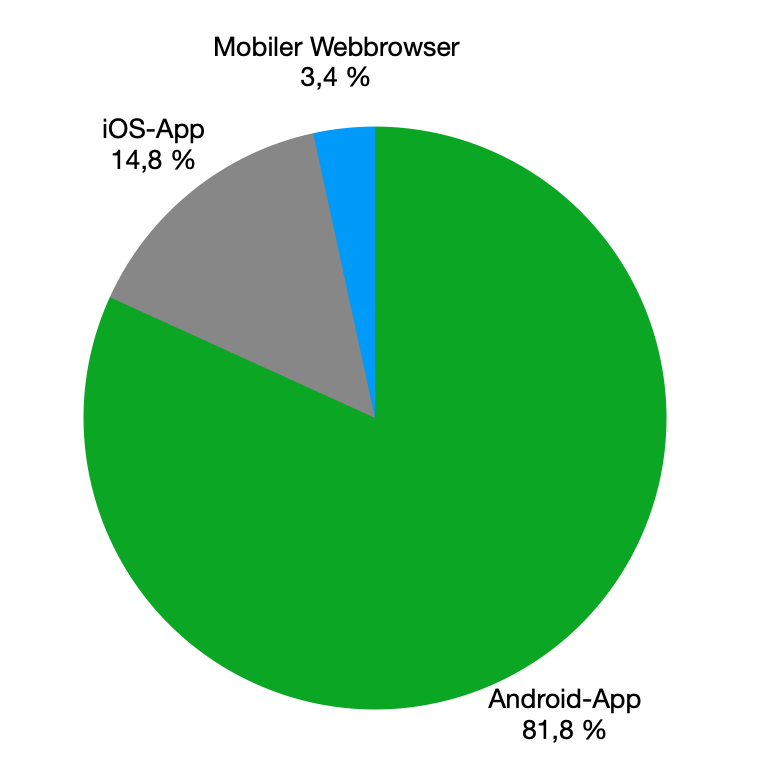
\includegraphics[scale=0.3]{_assets/facebook_mobile_users.png} \\
	Das Diagramm zeigt den deutlich dominierenden Anteil der Nutzenden von facebooks nativen Smartphone-Apps. Kombiniert kommen die Betriebssysteme Android und iOS auf einen Anteil von 96,6\%. Lediglich 3,4\% nutzen facebook auf dem Smartphone über einen Webbrowser \autocite{Kemp_Facebook}.
\end{figure}

Der große Anteil von Smartphone-Nutzenden im Vergleich zu Nutzenden von Desktops ist auf die Allgegenwärtigkeit von Smartphones zurückzuführen. Der Grund, weshalb Smartphone-Nutzende die native Anwendung präferieren, kann auf zwei Punkte zurückgeführt werden: Empfehlungen seitens facebook (siehe Anhang 2.1) und technische Vorteile. Der zweite Punkt lässt sich über beispielsweise Push-Mitteilungen erklären, welche aus dem Webbrowser nicht möglich sind. So wird den Konsumierenden eine direkte Kommunikation mit weiteren Nutzenden der Plattform vereinfacht. Da dieser Aspekt eng mit der User Experience der Nutzenden zusammenhängt, wird in dem gleichnamigen Absatz tiefer darauf eingegangen.

\subsubsection{User Experience}

Wie schon im Absatz zum Schaffen und Konsumieren von Inhalten, steht hier der Nutzende im Zentrum der Betrachtung. Als User Experience wird die Erfahrung eines Nutzenden zum Zeitpunkt der Interaktion mit der Software bezeichnet. Der Entwickelnde des Software kann über gezielten Einsatz von UI-Elementen und Plattformentscheidungen eine gute User Experience begünstigen, jedoch nicht erzwingen. Die User Experience als solches ist subjektiv und stark von dem Nutzenden und seiner Situation abhängig. \\
\textcite[28]{Jobe} gibt an, dass die Erfahrung der Nutzung der Software als Webanwendung aufgrund der limitierten Integrationsmöglichkeiten beschnitten wird. Er gibt weiterhin an, dass ohne externe Frameworks keine konkurrierende Nutzungserfahrung im Vergleich zu nativen Anwendungen geschaffen werden kann. Dies sieht der Autor in dem ungehinderten Zugang der nativen Software zur Hardware des Geräts, zu Interaktions- und Interface-Optionen der Hard- und Software begründet. \\

Angenommen, eine zu entwickelnde Webanwendung basiert auf Echtzeitkommunikation mit dem Nutzenden. Der Nutzende soll möglichst schnell über eine wichtige Information in Kenntnis gesetzt werden, weshalb sich die von Smartphones bekannte Interaktionsmöglichkeit der Push-Mitteilung anbieten würde. Tatsächlich existiert eine solche Möglichkeit über sogenannte Web Notifications. \\
Web Notifications erlauben die Interaktion mit dem Nutzenden über die native Benachrichtigungs-API des Betriebssystems, sogar wenn die Webanwendung nicht geöffnet ist. Um diese Technologie nutzen zu können, muss der Nutzende zunächst die Erlaubnis dazu geben \autocite{Notifications_API}. Dies ist jedoch an die Voraussetzung geknüpft, dass der Nutzende einen unterstützten Webbrowser benutzt:

\begin{table}[H]
 	\centering
 	\caption{Ausgewählte Browser mit Unterstützung für Web Notifications}
 	\begin{center}
 		\begin{tabularx}{\linewidth}{| Y | Y | Y |}
 			\hline
 			\textbf{Browser} & \textbf{Version} & \textbf{wird unterstützt} \\
 			\hline \hline
 			Internet Explorer & 11 & nein \\
 			\hline
 			Edge & 101 & ja \\
 			\hline
 			Firefox & 99 & ja \\
 			\hline
 			Chrome & 101 & ja \\
 			\hline
 			Safari & 15.4 & ja \\
 			\hline
 			Safari on iOS & 15.4 & nein \\
 			\hline
 			Android Browser & 101 & teilweise \\
 			\hline
 		\end{tabularx}
 	\end{center}
 	Die für native Anwendungen selbstverständliche Funktion, dem Nutzenden Push-Mitteilungen zukommen zu lassen, gestaltet sich für Webanwendungen eher schwierig. Begründet liegt dies in der mangelhaften Unterstützung insbesondere durch mobile Browser der Betriebssysteme iOS und Android \autocite{Web_Notifications}. 
 \end{table}

Prinzipiell ist diese Annäherung von Webanwendungen an Funktionalitäten nativer Anwendungen als positiver Aspekt für Webanwendungen zu sehen, jedoch können insbesondere Smartphones nicht einheitlich von diesem Feature profitieren. Um diese Funktion möglichst vorteilhaft zu nutzen, muss die Hard- und Software der Zielgruppe genau bestimmt werden. Sollte die Zielgruppe überwiegend Smartphones mit dem Browser \textit{Safari on iOS} nutzen, muss aufgrund von nicht vorhandenen Polyfills gänzlich auf dieses Feature der Webanwendung verzichtet werden. \\

Als weiterer Aspekt einer guten Nutzungserfahrung kann die Integration eines Kontextmenüs in die Webanwendung gesehen werden. Kontextmenüs sind ein natives Feature von vielen Desktop-Betriebssystemen und spiegeln ein gelerntes Verhalten des Nutzenden wieder. Eine Integration des Menüs in die Webanwendungen lässt die Grenzen zwischen nativen Anwendungen und Webanwendungen weiterhin verschwimmen. Auf diese Weise müssen Nutzende im Produktiveinsatz der Webanwendung keine neuen Arbeitsschritte lernen und profitieren von dem bereits gelernten Verhalten. Jedoch ist auch dieser Punkt uneinheitlich in den gängigen Webbrowsern integriert:

\begin{table}[H]
 	\centering
 	\caption{Ausgewählte Browser mit Unterstützung für das \texttt{contextmenu}-Event}
 	\begin{center}
 		\begin{tabularx}{\linewidth}{| Y | Y | Y |}
 			\hline
 			\textbf{Browser} & \textbf{Version} & \textbf{wird unterstützt} \\
 			\hline \hline
 			Internet Explorer & 11 & ja \\
 			\hline
 			Edge & 101 & ja \\
 			\hline
 			Firefox & 100 & ja \\
 			\hline
 			Chrome & 101 & ja \\
 			\hline
 			Safari & 15.4 & ja \\
 			\hline
 			Safari on iOS & 15.4 & nein \\
 			\hline
 			Android Browser & 101 & ja \\
 			\hline
 		\end{tabularx}
 	\end{center}
 	Die in Desktop-Browsern etablierte API für das \texttt{contextmenu}-Event wird sogar von Internet Explorer unterstützt, welcher von Entwickelnden aufgrund seiner unzureichenden Feature-Integration in der Regel lediglich durch Polyfills unterstützt wird. Einzig Safari on iOS unterstützt die genannte API nicht \autocite{contextmenu-event}. Dies hat zur Folge, dass das gelernte Verhalten der Nutzenden von Desktop-Systemen nicht auf die Nutzung von einem iPhone oder iPad projiziert werden kann.
 \end{table}
 
 Zur Schaffung einer möglichst positiven User Experience müssen sich Entwickelnde von Webanwendungen demnach vor der Entwicklung erkundigen, welche Hardware, beziehungsweise Software die Zielgruppe nutzt, um die Nutzungserfahrung über alle Browser gleich zu gestalten.

\subsubsection{Performanz}

Die Performanz von Webanwendungen bezeichnet \textcite[28]{Jobe} als abhängig von den genutzten Redering-Engines für HTML und JavaScript. Weiterhin sieht er die Leistung von Webanwendungen im Vergleich zu nativen Anwendungen durch den limitierten Zugriff auf die Hardware beschnitten. Hier erwähnt der Autor ausdrücklich die mangelhafte Leistung von Webbrowsern auf Smartphones. \\

Die Performanz einer Webanwendung ist im Wesentlichen durch die Performanz des genutzten Webbrowsers und nicht zuletzt durch die verfügbare Internetverbindung beschränkt. Somit scheint der Vergleich von nativen Anwendungen mit Webanwendungen in Hinblick auf die Leistungsfähigkeit nicht adäquat. Um dennoch den Evaluierungsprozess der Entwicklung anzudeuten, wird im Folgenden die Performanz der Rendering-Engines von Google Chrome und Safari verglichen. \\ 
Google Chrome nutzt für die Verarbeitung von JavaScript die sogenannte V8-Engine \autocite{v8_Engine}. Zur Darstellung von HTML nutzt Chrome ein Derivat der WebKit-Engine, die sogenannte Blink-Engine \autocite{Blink_Rendering}. \\
Safari hingegen nutzt für HTML und JavaScript die bereits erwähnte WebKit-Engine \autocite{WebKit}. \\
Um die Performanz der Browser zu testen und zu vergleichen, wird die Webanwendung \textit{speedometer} von \textit{browserbench} genutzt. Diese misst die Responsivität von einfachen Webanwendungen in dem genutzten Browser. Unter anderem nutzt die Webanwendungen \textit{Vue.js}, \textit{React}, \textit{Angular}. \textit{jQuery} und \textit{VanillaJS}. \\
Als Ergebnis des Tests erreicht Chrome durchschnittlich 104,9 Durchläufe pro Minute bei einer Standardabweichung von 3,39 über insgesamt 10 Versuchsdurchläufen. Safari hingegen erreicht durchschnittlich 129,1 Durchläufe pro Minute bei einer Standardabweichung von 4,25 über ebenfalls 10 Versuchsdurchläufe (siehe Anhang 1.3). Durchgeführt wird der Test auf einem MacBook Pro 2020 (siehe Anhang 1.2). \\
Als Resultat des Tests ist Safari performanter als Chrome. Diese Aussage ist jedoch nicht universell gültig, da hier lediglich ein Test genutzt wird, welcher auf lediglich einem Gerät durchgeführt wird. \\

\newpage

\subsection{Vor- und Nachteile von nativen Anwendungen}

Als nativ werden Anwendungen bezeichnet, welche speziell für eine Plattform entwickelt werden. Die zu verwendende Programmiersprache, Frameworks und Libraries sind maßgeblich von dem gewählten System abhängig. So sollte sich zum Beginn der Entwicklung die Frage gestellt werden, welche Plattform die angestrebte Zielgruppe nutzt:

\begin{table}[H]
 	\centering
 	\caption{Ausgewählte Betriebssysteme und die zugehörigen Programmiersprachen für native Entwicklung}
 	\begin{center}
 		\begin{tabularx}{\linewidth}{| Y | Y | Y |}
 			\hline
 			\textbf{Betriebssystem} & \textbf{Programmiersprache} & \textbf{Besonderheiten} \\
 			\hline \hline
 			Windows & Visual Basic. C\#, F\#, C++/CLI & .NET Framework zur Entwicklung und Ausführung \autocite{.NET_Microsoft} \\
 			\hline
 			MacOS, iOS und iPadOS & Swift & benötigt einen Mac zum Entwickeln \autocite{Swift_Apple} \\
 			\hline
 			Android & Kotlin & Java als Programmiersprache wird noch unterstützt, jedoch wird davon abgeraten \autocite{Kotlin_Android} \\
 			\hline
 			Linux & z.B. Python, C, C++, Rust, JavaScript & Stark abhängig von der gewählten Distribution, Einzelfallbetrachtung nötig \autocite{Linux_App} \\
 			\hline
 		\end{tabularx}
 	\end{center}
 	Native Anwendungen sollten möglichst nahe an dem Hostsystem geschrieben werden, um von möglichst großer Leistung zu profitieren. Die systemeingenen Sprachen ermöglichen dies ohne die Notwendigkeit für eine Runtime-Umgebung.
 \end{table}
 
 Einheitliche Eigenschaften von nativen Anwendungen sind uneingeschränkter Zugriff auf die vom Betriebssystem genehmigte Hardware und die Unterstützung für alle möglichen Interface- und Interaktions-Optionen des Geräts, beziehungsweise des Betriebssystems \autocite[28]{Jobe}. Eine weitere Gemeinsamkeit ist die Voraussetzung der Installation der Anwendung, um diese nutzen zu können. \\
 
 Welche Vor- und Nachteile die Entwicklung und Nutzung von nativen Anwendungen mit sich bringt, wird in den folgenden Absätzen erläutert. Hierzu wird sich erneut der Methodik von \textcite[28]{Jobe} bedient, welcher die Vor- und Nachteile nach den Gesichtspunkten Update-Frequenz, Entwicklung, Monetarisierung, Schaffen und Konsumieren von Inhalten, User Experience und Performanz. Im Kontext dieser Arbeit ist jedoch die Differenzierung zwischen mobilen Anwendungen und Desktop-Anwendungen besonders zu beachten. Letztere können von jeder Person entwickelt und veröffentlicht werden. Insbesondere iOS-Anwendungen hingegen können mit originaler iOS-Software lediglich aus dem App Store herunter geladen werden. Auf diese Weise wirkt Apple Kontrolle und Regulierungen aus, um beispielsweise Schadsoftware für iOS-Nutzende unzugänglich zu machen \autocite{Appstore_Guildelines}.


\subsubsection{Update-Frequenz}

Begonnen mit der Betrachtung von Anwendungen, welche über einen Store, wie beispielsweise Apples App Store, Googles Play Store oder der Microsoft Store, veröffentlicht werden, sind Aktualisierungen der Anwendungen formal über die integrierte Funktion des Stores \autocite[28]{Jobe}. Als stellvertretendes Beispiel wird hier Apples App Store angeführt. Die Aussagen gelten dabei für mobile Apps unter iOS und iPadOS, aber auch für Desktop-Anwendungen über den MacOS App Store. Diese verfügen unter anderem über einen ausführlichen Workflow für das Aktualisieren einer Anwendung. Dabei kann die Entwicklerin oder der Entwickler einen Change-Log führen, den Nutzenden über Änderungen in den Nutzungsbedingungen informieren oder Plattform-Unterstützung direkt auf der Seite der Anwendung im Store angeben \autocite{Appstore_Updates}. \\
Diese Dienstleistung seitens Apple ist für Nutzende und für Entwickelnde von Vorteil. Nutzende sehen auf einen Blick Änderungen, Neuigkeiten und unterstützte Plattformen der Anwendung. Entwickelnde müssen so keine gesonderten rechtlichen Texte, Change-Logs oder Ähnliches in die Anwendung integrieren, sondern können sich auf das Schaffen einer angenehmen User Experience fokussieren. \\

Anwendungen hingegen, welche nicht über Stores veröffentlicht werden, können beispielsweise über das Internet heruntergeladen werden. Diese sind in der Regel nicht reguliert. Daraus resultierend haben Entwickelnde dieser Anwendungen keinerlei Verpflichtungen gegenüber einer Plattform. Dadurch werden uneinheitliche Praktiken angewandt, wodurch die User Experience noch vor der Installation verglichen mit einem Download aus einem Store vergleichsweise gering ausfallen kann. 


\subsubsection{Entwicklung}

Die Entwicklung von nativen Anwendungen ist äußerst abhängig von der Plattform. Die Wahl von Frameworks, Libraries und Programmiersprachen kann erst nach der Entscheidung für die Plattform getroffen werden. Welche Hindernisse eine Entwicklerin oder ein Entwickler dabei bewältigen muss, wird in diesem Abschnitt näher beleuchtet. \\
Ein ausschlaggebender Zeitpunkt im Entwicklungsprozess ist die Wahl der Plattform. Entwickelnde können sich bei der Wahl beispielsweise folgende Fragen stellen: 

\begin{itemize}
	\item Soll die Anwendung über einen der bereits erwähnten Stores zur Verfügung gestellt werden?
	\item Soll die Andendung nur auf einem bestimmten Gerät ausführbar sein?
	\item Unterstützt die angestrebte Hardware, beziehungsweise das Betriebssystem die Anforderungen der Anwendungen?
\end{itemize}

Benötigen Entwickelnde beispielsweise einen hardwareseitig verbauten Gyroskopsensor und die zugehörige API für die Anwendung, so sollten sie ein Smartphone als Endgerät in Betracht ziehen. Hat das Entwicklungsteam keinen Zugriff auf einem Mac, so sollte auf die Entwicklung der Anwendung für Apples Betriebssysteme verzichtet werden. \\
Ebenfalls zu berücksichtigen sind die zahlreichen Formfaktoren der Displays moderner Endgeräte. Die Displays von modernen Smartphones sind nicht länger rechteckig, weisen Aussparungen für Kameras und Sensoren auf und sind teilweise sogar faltbar.

\begin{figure}[H]
	\centering
	\caption{Ausgewählte Endgeräte mit unregelmäßigen Displayformaten}
	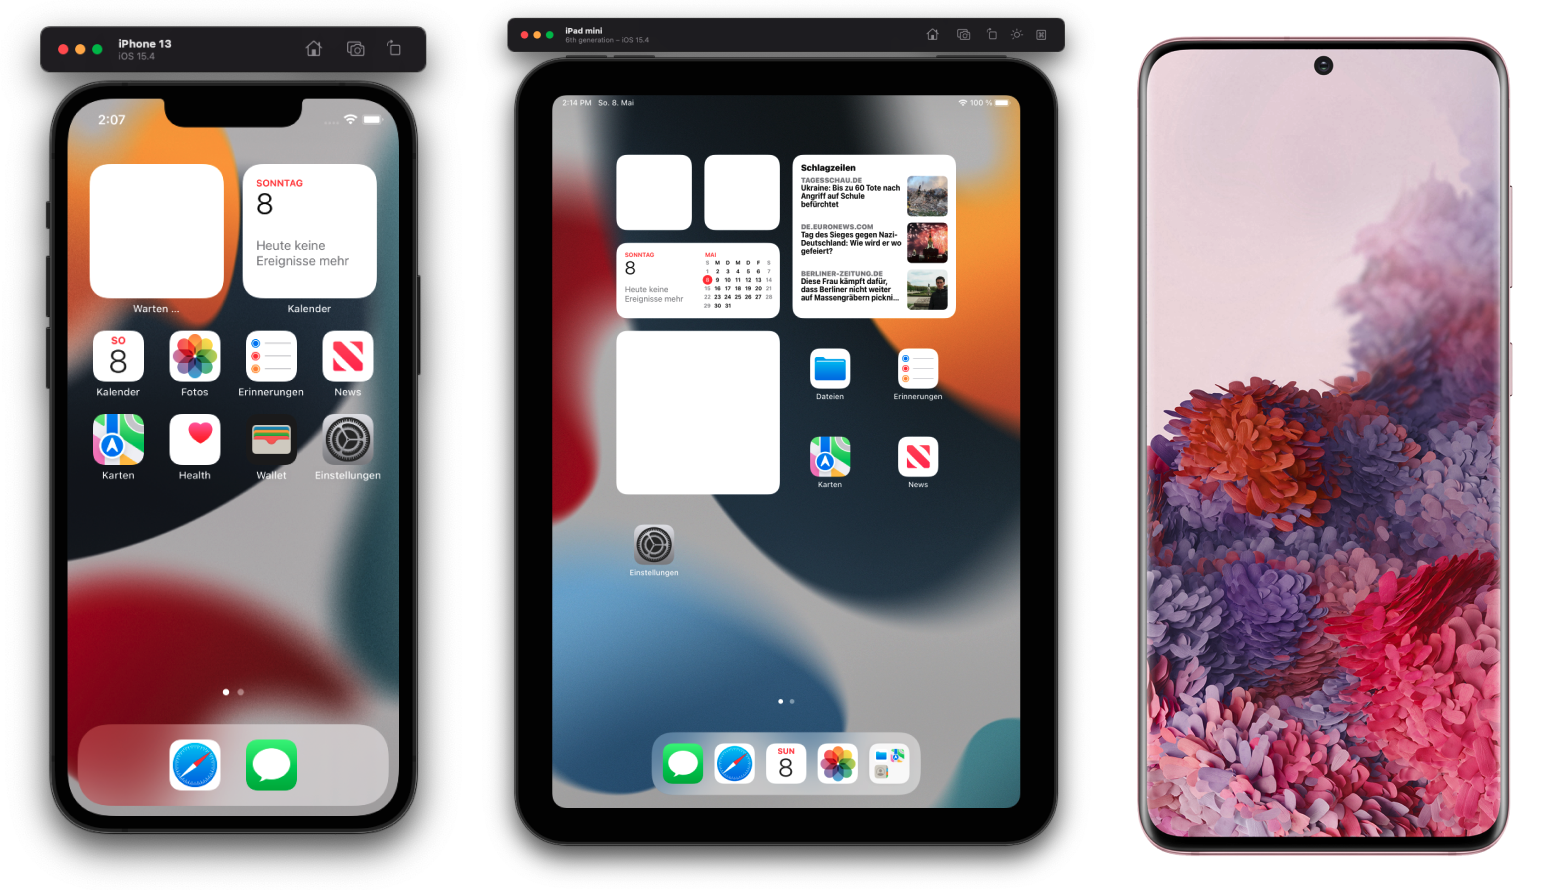
\includegraphics[scale=0.25]{_assets/phones_displays.png} \\
	Bei den hier gezeigten Geräten handelt es sich um das Apple iPhone 13, das Apple iPad mini und das Samsung Galaxy S20 \autocite{Galaxy_Picture}. Alle Geräte verfügen über abgerundete Ecken und die Smartphones zeigen zusätzliche Aussparungen im Display für Kameras und Sensorik.
\end{figure}

Dieser Trend von unregelmäßigen Displayformaten ist spätestens mit der Veröffentlichung von Apples MacBook Pro 2021 auf ein Notebook übergesprungen.

\begin{figure}[H]
	\centering
	\caption{Das Display von Apples MacBook Pro 2021}
	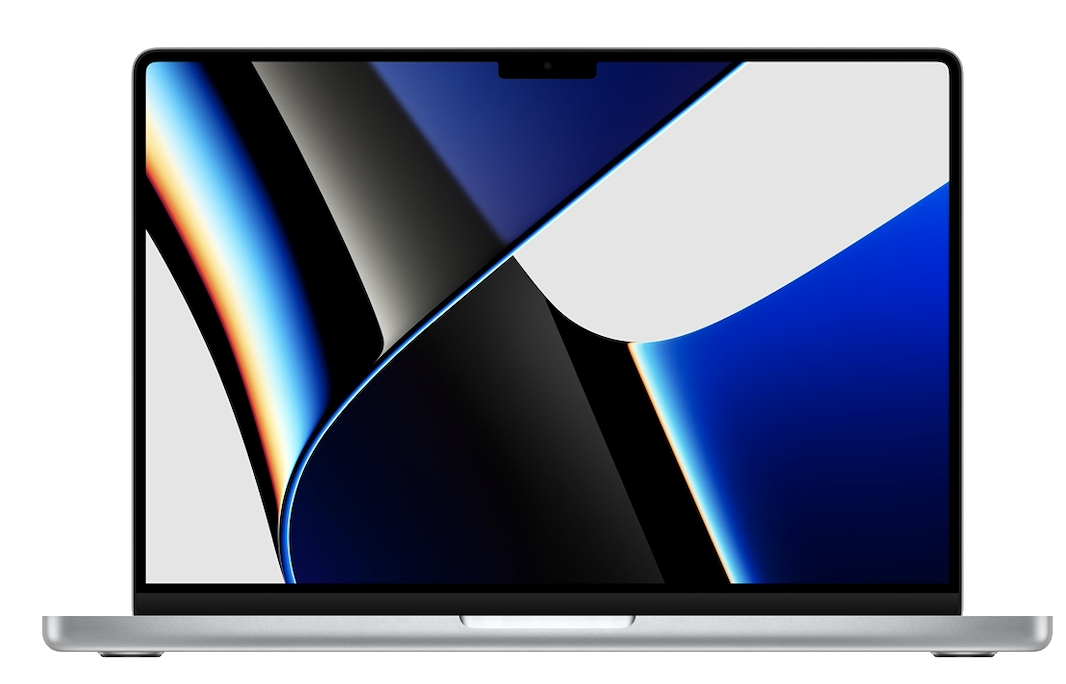
\includegraphics[scale=0.25]{_assets/macbook_display.png} \\
	Apple etabliert mit der Veröffentlichung des MacBook Pro 2021 abgerundete Ecken und Aussparungen im Display ihrer Notebooks \autocite{Macbook_Display}. Besonders zu beachten ist, dass nur die oberen Ecken des Displays abgerundet sind. Die unteren Ecken verbleiben rechteckig.
\end{figure}

Inwiefern dies die User Experience verändert, wird in einem späteren Abschnitt beleuchtet. Der direkte Einfluss auf die Entwicklung ist jedoch unabstreitbar. Es kann nicht länger von einem rechteckigen zweidimensionalen Viewport ausgegangen werden. Faltbare Smartphones, gebogene Displays unregelmäßige Aussparungen gehören zu modernen Smartphones dazu. Die etablierten Entwicklungsumgebungen, am Beispiel von Xcode, erleichtern das Berücksichtigen dieser Sonderfälle. Dies hat jedoch zur Folge, dass UI-Elemente entweder verdeckt und unerreichbar sind, oder sie für jedes unterstützte Gerät neu positioniert werden müssen. Vergleichbar ist diese Problematik mit responsive Design von Websites. \\
In dem Fall einer Webentwicklung haben Entwickelnde die Möglichkeit, über das CSS-Feature \texttt{@media} CSS-Regeln anzuwenden, wenn einen gegebene Bedingung wahr ist. So lassen sich beispielsweise Höhe und Breite des Viewports abfragen, wodurch das Design der Webanwendung sich einem kleinen Smartphone-Viewport oder einem großen Desktop-Viewport anpassen kann \autocite{Media_Queries}. \\

Ein weiterer, nicht zu vernachlässigender Aspekt der nativen Entwicklung ist der Mehraufwand bei einer Unterstützung von mehr als einer Plattform. Soll die Anwendung für Nutzerinnen und Nutzer auf verschiedenen Betriebssystemen verfügbar sein, muss die Anwendung mehrmals nativ entwickelt und veröffentlicht werden. Dazu sind unterschiedliche Programmiersprachen, Frameworks und IDEs nötig, was zusätzlichen Lernaufwand bedeutet, sollten die Grundlagen hierzu erst erschlossen werden müssen. \\

Als finaler Punkt sei hier die ungleichmäßige Integration von Hardware-APIs angeführt. Insbesondere Smartphones profitieren von einer Vielzahl von Sensoren, auf welche eine Anwendung Zugriff haben kann. Stellvertretend sei hier Apples iPhone 13 Pro aufgeführt, welches über Apples eigene Gesichtserkennungstechnologie Face ID, einen LiDAR Scanner, ein Barometer, einen 3-Achsen Gyrosensor, einen Beschleunigungssensor und mehr verfügt \autocite{iPhone13_specs}. Diese Sensoren sind jedoch in älteren Smartphones von Apple nicht verbaut, wodurch die potenzielle Zielgruppe schrumpft. Als Folge dessen müssen Entwickelnde nicht nur Hardware-Abfragen bei Smartphones unterschiedlicher Hersteller beachten, sondern ebenfalls die Klientel mit älteren Smartphones einer identischen Marke berücksichtigen.


\subsubsection{Monetarisierung}

Die Monetarisierung von nativen Anwendungen in Stores ist über die Stores selbst möglich \autocite{Appstore_Connect}. Dabei wird den Entwickelnden selbst überlassen, ob die Anwendung einmalig Geld kosten soll, eine wiederkehrende Summe verlangt wird oder Werbung geschaltet wird. \\
Werden hingegen native Anwendungen betrachtet, die nicht durch Stores verwaltet werden, müssen sich Entwickelnde selbst um eine Zahlungsintegration bemühen. Hier genießen Entwickelnde, vergleichbar mit der Monetarisierung von Webanwendungen, vollkommene Freiheit.


\subsubsection{Schaffen und Konsumieren von Inhalten}

\textcite[28]{Jobe} sieht native Anwendungen im Aspekt des Schaffens von Inhalten im Vorteil. In dem vorigen Abschnitt zu Webanwendungen und deren Möglichkeiten zum Schaffen und Konsumieren von Inhalten wird festgestellt, dass native Anwendungen sowohl das Schaffen als auch das Konsumieren von Webanwendungen vereinfachen, beziehungsweise Nutzende die native Option von Anwendungen Webanwendungen vorziehen. Genauer wird dieser Aspekt in dem Abschnitt Performanz beleuchtet.


\subsubsection{User Experience}

Die Nutzungserfahrung von nativen Anwendungen wird nicht zuletzt durch den Aspekt der nativen Performanz und direktem Hardware-Zugriff begünstigt. \textcite[28]{Jobe} begründet die Überlegenheit von nativen Anwendungen im Punkto User Experience mit einer nahtlosen Integration der Software in das Betriebssystem. So ist es möglich, dass Entwickelnde User-Interface-Elemente des Betriebssystems nutzen können. Das gelernte Verhalten dieser Elemente fördert eine positive Erfahrung der Nutzenden, sodass diese keine neuen Design-Sprachen lernen müssen. \\
\textcite[1001]{native_vs_web} beleuchten in ihrer Arbeit die Performanz von nativen Anwendung und Webanwendungen basierend auf dem Android Betriebssystem. Hier erwähnen die Autoren, dass die Möglichkeiten nativer Anwendungen einen Vergleich dieser Ansätze ungerecht aussehen lassen. So verfügen native Anwendungen über die Möglichkeit, Einstellungen der Geräte kontextbezogen anzupassen. Als Beispiele werden Limitation des Stromkonsums bei schwacher Batterieleistung, Einschränkung des Datenverkehrs bei geringer Konnektivität und das softwareseitige Verbieten von umfangreichen Downloads ohne WLAN-Verbindung. \\
Diese Möglichkeiten von nativen Anwendungen können die User Experience verbessern. Native Anwendungen dominieren in diesem Aspekt Webanwendungen aufgrund des uneingeschränkten Zugriffs auf verbaute Sensoren und das Betriebssystem.

\subsubsection{Performanz}

Native Anwendungen ziehen ihre Vorteile nicht nur aus dem Zugriff auf Informationen der Sensoren, sondern auch aus der hohen Performanz im Vergleich zu Webanwendungen. Wie bereits in der Betrachtung von Webanwendungen erwähnt, ist die Performanz von Webanwendungen durch die Performanz der durch den Browser genutzten Rendering Engines beschränkt. Native Anwendungen hingegen werden nicht von einer solchen Abstraktionsschicht eingeschränkt, wodurch ihre Performanz lediglich durch das Betriebssystem und die verbaute Hardware limitiert ist \textcite[28]{Jobe}. \\
In der Arbeit von \textcite[999]{native_vs_web} wird dieser Aspekt im Kontext von Smartphones genauer beleuchtet. Die Autoren finden heraus, dass native Anwendungen verglichen mit Webanwendungen im allgemeinen weniger Daten übertragen. Dies sehen die Autoren in der Möglichkeit der programmatischen Limitierung der Anzahl und Größe der heruntergeladenen Ressourcen durch native Entwickelnde begründet. Weiterhin wird nativen Entwickelnden die Freiheit gelassen, selbst über Daten im Cache zu verwalten. Diese Option wird im Fall von Webanwendungen gänzlich dem Browser überlassen. \textcite[999]{native_vs_web} bewerten die Cache-Funktion von insbesondere mobilen Browsern als nicht zufriedenstellend. Als Gründe geben die Autoren unter anderem redundante Übertragungen von Daten an. Sie beschreiben weiterhin die mangelhafte Optimierung von Websites als einen primären Grund für die mangelhafte Cache-Performanz von Webanwendungen. Mittels kontextbezogener Anpassungen der Anfragen nach Ressourcen der Webanwendungen, lassen sich diese, so die Autoren, auf dieselbe Cache-Performanz bringen, wie sie native Anwendungen aufweisen. \\
Die stellvertretend betrachtete Cache-Performanz von nativen Smartphone-Anwendungen überwiegt demnach in der Regel die von mobilen Webanwendungen, wie auch \textcite[1]{Beyond_native_apps} bestätigt.

\newpage

\subsection{Cross-Plattform}

Die Entwicklung von Cross-Plattform-Anwendungen ist kein neues Phänomen. Der Ansatz von Cross-Kompilierung erlaubt Entwickelnden, die gewünschte Anwendung in einer kompilierten Programmiersprache zu entwicklen und diese unabhängig für unterschiedliche Plattformen zu kompilieren. Dies reduziert den Aufwand, den kompilierten plattform-nativen Code individuell zu entwickeln \autocite[7]{Xamarin}. \\
Prinzipiell besitzen CP-Anwendungen vergleichbare Vorteile gegenüber Webanwendungen, wie sie native Anwendungen gegenüber Webanwendungen aufweisen. Begründet liegt dies in dem bereits erwähnten kompilierten nativen Code für die jeweilige Plattform. Werden jedoch CP-Anwendungen mit nativ Entwickelten Anwendungen verglichen, werden Unterschiede deutlich. \textcite[7]{Xamarin} erwähnt eine geringe Performanz bei einem Vergleich mit nativen Anwendungen. Dies sieht der Autor in der Menge von Libraries begründet, welche in dem Speicher abgelegt werden müssen. Dieser Vergleich hängt jedoch stark von dem verwendetem CP-Framework ab, wie \textcite[134]{CP-mobile} bei dem Vergleich der Performanz von nativen mobilen Anwendungen mit Anwendungen des CP-Frameworks \textit{PhoneGap} angeben. \\
Wie bei jeder Entwicklung müssen sich Entwickelnde zunächst über die Zielgruppe informieren. Die genutzte Hard- und Software der Zielgruppe entscheidet maßgeblich über die Wahl des Frameworks und somit auch über die zu nutzende Programmiersprache. Die Betrachtung der hier aufgeführten Frameworks wird vor dem Hintergrund eines Web-Entwickelnden mit einer Expertise in dem Web-Framework React durchgeführt. Dieser Hintergrund wird im Praxis-Teil dieser Arbeit erneut aufgegriffen, wenn die Frameworks zur Entwicklung von spezifischen Anwendungen genutzt werden.

\subsubsection{Unterstützte Plattformen}

Wie bereits erwähnt, ist die Plattform der Zielgruppe maßgeblich bestimmend für das zu nutzende CP-Framework. Ist die Zielgruppe eher auf mobilen Systemen aktiv, sollte ein Framework wie React Native in Betracht gezogen werden, welches primär auf iOS/iPadOS und Android ausgelegt ist \autocite{React_Native}. Sollte sich die Zielgruppe eher an Desktop-Systemen finden, lohnt sich die Evaluierung des Frameworks Eletron \autocite{Electron.js}. Electron nutzt die Webtechnologien HTML, CSS und JavaScript und kompiliert für MacOS, Windows oder Linux eine native Anwendung aus einer gemeinsamen Code-Basis. Kennen die Entwickelnden ihre Zielgruppe nicht, so lohnt sich eine Betrachtung des Frameworks Flutter. Flutter ist ein CP-Framework zur Erstellung von nativen Anwendungen aus einer gemeinsamen Code-Basis für eine große Menge unterschiedlicher Plattformen. Dazu zählen mobile Plattformen, das Web, Desktop-Plattformen und sogar Embedded Systems \autocite{Flutter}. Die hier erwähnten Frameworks werden im Folgenden genauere Betrachtung finden.

\subsubsection{Gängige Frameworks}

React Native und Flutter belegen in der Stackoverflow Umfrage aus 2021 den sechsten und siebten Platz der beliebtesten Frameworks von etwas unter 60.000 Befragten \autocite{stackoverflow_2021}. Um ebenfalls ein rein desktop-orientiertes CP-Framework einzubringen, wird Electron hier Erwähnung finden.

\paragraph{React Native}

React Native ist ein von Facebook im Jahr 2015 veröffentlichtes CP-Framework zur Entwicklung von mobilen Anwendungen. React Native setzt, wie React auch, auf einen abgewandelten JavaScript-Syntax namens JSX. Zusätzlich kann CSS, beziehungsweise ein CSS-Preprozessor für Styling angewendet werden. React als Web-Framework kompiliert den geschriebenen Code und gibt die Komponenten an das Browser DOM weiter. So wird der geschriebene Code in HTML, CSS und clientseitiges JavaScript ausgegeben. React Native hingegen respektiert und berücksichtigt die nativen UI-Elemente und UX-Entscheidungen der Betriebssysteme. So werden JSX-Komponenten über eine sogenannte Bridge zu nativen Komponenten des jeweiligen Betriebssystems kompiliert \autocite[10f.]{React_Native_Danielsson}. \\
Als Resultat dessen weisen Anwendungen, welche in React Native entwickelt werden, eine gute Integration in die Design-Sprache des Host-Systems auf.

\paragraph{Electron}

Electron ist ein Framework, mit welchem Entwickelnde native Desktop-Anwendungen mithilfe von Webtechnologien entwickeln können. Zu den Ziel-Betriebssystemen zählen MacOS, Windows und Linux. Bekannte Programme, welche Electron nutzen, sind beispielsweise Visual Studio Code, Microsoft Teams oder WhatsApp \autocite{Electron.js}. Electron basiert auf Chromium und Node.js und vereint diese Technologien in einem Framework \autocite[Jasim 2017, zitiert nach][572]{Electron_Kredpattanakul}. \\

\paragraph{Flutter}

Flutter sticht als Framework in dieser Aufzählung etwas heraus. Primär liegt dies daran, dass Webentwickelnde für dieses Framework nicht die üblichen Technologien HTML, CSS und JavaScript nutzen können, sondern sich gegebenenfalls den Dart-Syntax aneignen müssen. Wie eingangs erwähnt, ist Flutter ein Cross-Plattform-Framework zur Entwicklung von nativen Anwendungen auf mobilen Systemen, Desktop-Systemen, Embedded Systems und sogar Webanwendungen \autocite{Flutter}. Damit deckt Flutter in dieser Aufzählung die meisten Plattformen ab, was den Grund für die Aufnahme des Frameworks in diese Arbeit darstellt.

\newpage

\section{Praktischer Vergleich von Cross-Plattform-Lösungen}

Die erarbeitete Theorie wird an Beispielen von hierfür entwickelten Anwendungen gezeigt. Dazu werden die bereits beleuchteten Cross-Plattform-Frameworks React Native, Electron und Flutter genutzt. Hierbei ist zu erwähnen, dass sich der Hintergrund des Autors fast ausschließlich auf die Entwicklung von Webanwendungen bezieht. Sämtliches Wissen über die Frameworks wird sich speziell für diese Arbeit zugelegt. Dabei spielt Flutter durch die Dart-Programmiersprache eine besondere Rolle, da hierfür die Grundlagen des Frameworks und der Sprache erlernt werden müssen.

\subsection{Zielvorgabe}

Es sollen Anwendungen entwickelt werden, welche auf die Plattformen MacOS, Windows, Linux, iOS, Android und das Web ausgelegt sind. Dazu sollen die von den Frameworks „out-of-the-box“ unterstützen Plattformen gezielt angesprochen werden. Externe Packeges, welche Unterstützung für weitere Plattformen nachrüsten, werden hier nicht betrachtet. Für React Native wird Expo genutzt, um die Entwicklung zu vereinfachen. Tabellarisch ausgedrückt unterstützen die jeweiligen CP-Frameworks die folgenden Plattformen:

\begin{table}[H]
 	\centering
 	\caption{Ausgewählte Cross-Plattform-Frameworks und ihre Zielplattformen}
 	\begin{center}
 		\begin{tabular}{| l || c | c | c | c | c | c |}
 			\hline
 			\textbf{} & \textbf{MacOS} & \textbf{Windows} & \textbf{Linux} & \textbf{iOS} & \textbf{Android} & \textbf{Web} \\
 			\hline \hline
			\textbf{React Native} & \xmark & \xmark & \xmark & \Checkmark & \Checkmark & \xmark \\
 			\hline
 			\textbf{Electron} & \Checkmark & \Checkmark & \Checkmark & \xmark & \xmark & \xmark \\
 			\hline
 			\textbf{Flutter} & \Checkmark & \Checkmark & \Checkmark & \Checkmark & \Checkmark & \Checkmark \\
 			\hline
 		\end{tabular}
 	\end{center}
	Unterstützung der Cross-Plattform-Frameworks für die einzelnen Plattformen. Flutter unterstützt zuzüglich Embedded Systems, welche jedoch aufgrund von mangelnder Relevanz keine Betrachtung finden.
 \end{table}
 
 Die Zielsysteme werden aufgrund mangelnder Geräte teilweise virtualisiert, beziehungsweise simuliert. Die folgenden Versionen der Plattformen werden genutzt:
 
\begin{table}[H]
 	\centering
 	\caption{Versionen der Zielbetriebssysteme}
 	\begin{center}
 		\begin{tabularx}{\linewidth}{| Y | Y | c |}
 			\hline
 			\textbf{Betriebssystem} & \textbf{Version} & \textbf{virtualisiert/simuliert} \\
 			\hline \hline
			MacOS & MacOS Monterey Version 12.3.1 (Hardware siehe Anhang 1.2) & \xmark \\
 			\hline
 			Windows & Windows 10 Home Version 21H2 (Hardware siehe Anhang 1.4) & \xmark \\
 			\hline
 			Linux & Ubuntu 22.04 LTS & \Checkmark \\
 			\hline
 			iOS & iOS 15.4.1 & \xmark \\
 			\hline
 			Android & Andoid 8.1 Oreo & \Checkmark \\
 			\hline
 			Web & Chrome Version 101.0.4951.54 for MacOS & \xmark \\
 			\hline
 		\end{tabularx}
 	\end{center}
	Für den Test mit iOS wird ein Apple iPhone XS und für Android ein simuliertes Google Pixel 4 genutzt. Die Virtualisierung der Linux-Distribution wird mithilfe von VirtualBox Version 6.1 durchgeführt.
\end{table}
 
Folgende Elemente sollen in die zu entwickelnden Anwendungen integriert werden:

\begin{itemize}
	\item eine Textanzeige über den aktuellen Status der Energieversorgung des Gerätes
	\item eine Textanzeige über die aktuelle Ausrichtung des Gerätes
	\item eine Umrandung des Viewports
	\item ein nativer Button, welcher eine Mitteilung über das native Mitteilungssystem auslöst 
\end{itemize}

Über die Textanzeigen wird de Zugriff der Anwendungen auf die Sensor-APIs geprüft. Die Umrandung des Viewports dient der Visualisierung einer möglichen Integration nicht-rechteckiger Displays in das Framework, der Button prüft die Verfügbarkeit nativer UI-Elemente und die Mitteilung testet die Integration nativer Mitteilungen in dem Framework. Das Styling der Anwendungen wird auf ein Minimum reduziert, da der Fokus auf der Funktionalität liegt. \\
Zur genaueren Visualisierung soll folgendes MockUp dienen:

\begin{figure}[H]
	\centering
	\caption{MockUp der zu entwickelnden Anwendung}
	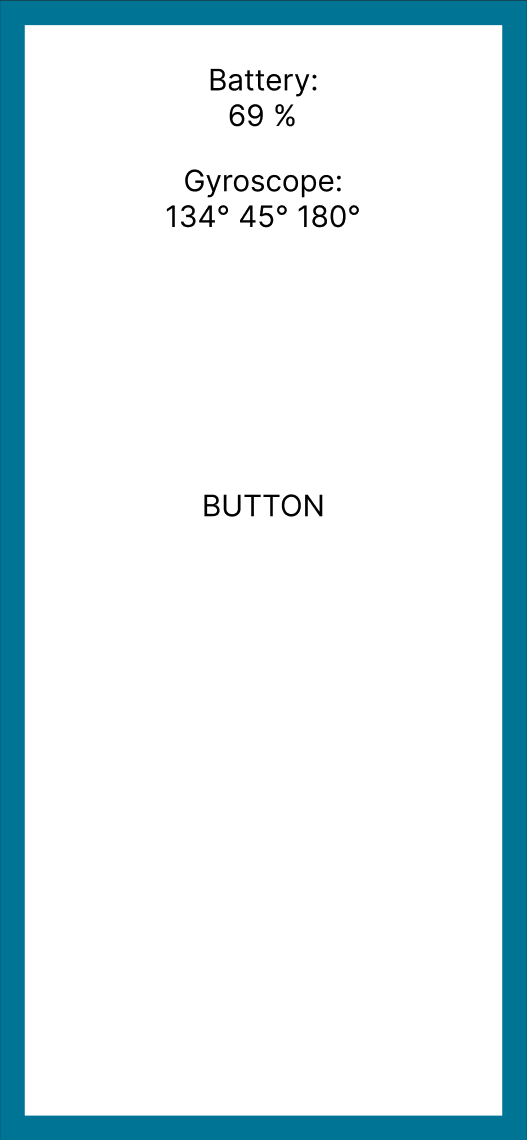
\includegraphics[scale=0.28]{_assets/MockUp.png} \\
	Das MockUp zeigt die grundlegend umzusetzenden Anforderungen. Werte und Anordnung dienen hier als Orientierung und können sich während der Entwicklung ändern.
\end{figure}

 
\subsection{Vergleich der Umsetzungen}

\section{Diskussion}

\subsection{Beleg der Hypothese}

\subsection{Limitation}

\subsection{Ausblick}

\section{Fazit}

% ---------------------
% Literaturverzeichnis:
% ---------------------

% Neue Seite beginnen:
\newpage

% Seitenzahl als römische Zahl angeben:
\pagenumbering{Roman}

% Beginn der Zählung bei 5:
\setcounter{page}{6}

% Literaturverzeichnis zu TOC hinzufügen:
\addcontentsline{toc}{section}{Liteaturverzeichnis}

% Literaturverzeichnis:
\section*{Literaturverzeichnis}

% Einfacher Zeilenabstand:
\singlespacing

% Literaturverzeichnis rendern

\printbibliography[heading=none]

\newpage

% --------------------------
% Eidesstattliche Erklärung:
% --------------------------

% Neue Section:
\section*{Eidesstattliche Erklärung}

\addcontentsline{toc}{section}{Eidesstattliche Erklärung}

% 1,5-facher Zeilenabstand:
\onehalfspacing

Ich erkläre hiermit und versichere an Eides Statt, dass ich meine Bachelor-Thesis / mein Praxisprojekt „Chancen und Risiken einer Migration von Webanwendungen zu nativen Systemen“ selbständig und ohne fremde Hilfe angefertigt habe und dass ich alle von anderen Autoren wörtlich übernommenen Stellen wie auch die sich an Gedankengänge anderer Autoren eng anlehnenden Ausführungen meiner Arbeit besonders gekennzeichnet und die Quellen zitiert habe. \\
Des Weiteren erkläre ich, dass sämtliche Ausführungen nicht bereits inhaltlicher Bestandteil einer anderen Prüfungsleistung (z.B. Praxisprojekte, Semesterarbeiten) gewesen sind. \\
Mir ist bekannt, dass bei einem Verstoß gegen diese Erklärung die Prüfungsleistung mit der Note „nicht ausreichend“ bewertet wird. \\ \\

Kiel, den 16.05.2022 \\ \\ 

% Tabbing-Umgebung für Unterschriften:
\begin{tabbing}
	\_\_\_\_\_\_\_\_\_\_\_\_\_\_\_\_\_\_\_\_\_\_\_\_\_ \\
	Fabian Reitz
\end{tabbing}

% -------
% Anhang:
% -------

% Neue Seite beginnen:
\newpage

\appendix

\section*{Anhang}
\addcontentsline{toc}{section}{Anhang}

\subsection*{Anhang 1: Tabellen}
\addcontentsline{toc}{subsection}{Anhang 1: Tabellen}

\subsubsection*{Anhang 1.1: stackoverflow Developer Surveys 2015 bis 2021}
\addcontentsline{toc}{subsubsection}{Anhang 1.1: stackoverflow Developer Surveys 2015 bis 2021}

\begin{table}[H]
	\centering
	\caption{Anzahl der Antworten der stackoverflow Developer Surveys 2015 bis 2021}
	\begin{center}
		\begin{tabular}{| l | c | c |}
			\hline
			Jahr & Absolute Anzahl aller Antworten & Relativer Anteil Full-Stack Developer \\
			\hline \hline
			2013 & 8.218 Antworten & 29 \% \\
			\hline
			2014 & 7.346 Antworten & 26,8 \% \\
			\hline
			2015 & 22.148 Antworten & 32,4 \% \\
			\hline 
			2016 & 49.525 Antworten & 28 \% \\
			\hline 
			2017 & 36.125 Antworten & 46,3 \% \\
			\hline 
			2018 & 92.098 Antworten & 48,2 \% \\
			\hline
			2019 & 81.335 Antworten & 51,9 \% \\
			\hline
			2020 & 49.370 Antworten & 54,9 \% \\
			\hline
			2021 & 66.484 Antworten & 49,5 \% \\
			\hline
		\end{tabular}
	\end{center}
	Die Tabelle zeigt die Anzahl aller Antworten pro Jahr der \textit{stackoverflow Developer Survey}, sowie den relativen Anteil von Full-Stack Developern an diesen Antworten \autocite{stackoverflow_2015,stackoverflow_2016,stackoverflow_2017,stackoverflow_2018,stackoverflow_2019,stackoverflow_2020,stackoverflow_2021}.
\end{table}

\newpage

\subsubsection*{Anhang 1.2: Hard- und Softwarespezifikationen des Testsystemes}
\addcontentsline{toc}{subsubsection}{Anhang 1.2: Hard- und Softwarespezifikationen des Testsystemes}

\begin{table}[H]
	\centering
	\caption{Hard- und Softwarespezifikationen des Testsystemes für den Vergleich der Leistungsfähigkeit von Safari und Chrome}
	\begin{center}
		\begin{tabularx}{\linewidth}{| l | X |}
			\hline
			Aspekt & System \\ 
			\hline \hline
			Betriebssystem & macOS Monterey Version 12.3.1 \\
			\hline
			Chrome Version & Version 100.0.4896.127 (Offizieller Build) (x86\_64) \\
			\hline
			Safari Version & Version 15.4 (17613.1.17.1.13) \\
			\hline
			Modell & MacBook Pro (13 Zoll, 2020, Vier Thunderbolt 3 Anschlüsse) \\
			\hline
			Prozessor & 2 GHz Quad-Core Intel Core i5 \\
			\hline
			Speicher & 32 GB 3.733 MHz LPDDR4X \\
			\hline
			Grafikkarte & Intel Iris Plus Graphics 1.536 MB \\
			\hline
		\end{tabularx}
	\end{center}
	Das hier aufgeschlüsselte System wird zum Testen der Browser-Responsivität genutzt.
\end{table}

\newpage

\subsubsection*{Anhang 1.3: Ergebnisse des Tests zur Erfassung der Browser-Responsivität von Safari und Chrome}
\addcontentsline{toc}{subsubsection}{Anhang 1.3: Ergebnisse des Tests zur Erfassung der Browser-Responsivität von Safari und Chrome}

\begin{table}[H]
	\centering
	\caption{Ergebnisse des Tests zur Erfassung der Browser-Responsivität von Safari und Chrome mittels \textit{speedometer}}
	\begin{center}
		\begin{tabularx}{\linewidth}{| l || X | X |}
			\hline
			Durchlauf & Chrome & Safari \\ 
			\hline \hline
			1. Durchlauf & 108 (\( \pm \)1,6) & 131 (\( \pm \)3,4) \\
			\hline
			2. Durchlauf & 107 (\( \pm \)2,3) & 125 (\( \pm \)3,4) \\
			\hline
			3. Durchlauf & 109 (\( \pm \)5,8 ) & 139 (\( \pm \)3,5) \\
			\hline
			4. Durchlauf & 106 (\( \pm \)1,6) & 123 (\( \pm \)9,0) \\
			\hline
			5. Durchlauf & 111 (\( \pm \)5,3) & 130 (\( \pm \)1,4) \\
			\hline
			6. Durchlauf & 103 (\( \pm \)3,1) & 128 (\( \pm \)2,5) \\
			\hline
			7. Durchlauf & 103 (\( \pm \)2,9) & 129 (\( \pm \)2,4) \\
			\hline
			8. Durchlauf & 99 (\( \pm \)4,7) & 127 (\( \pm \)2,1) \\
			\hline
			9. Durchlauf & 103 (\( \pm \)1,8) & 130 (\( \pm \)3,1) \\
			\hline
			10. Durchlauf & 100 (\( \pm \)3,4) & 129 (\( \pm \)4,0) \\
			\hline \hline
			Mittelwert & 104,9 (gesamt\( \pm \)3,93) & 129,1 (gesamt\( \pm \)4,25) \\ 
			\hline
		\end{tabularx}
	\end{center}
	Dies sind die Testergebnisse des Browser-Responsivität, ermittelt mit \textit{speedometer}. Die Angaben sind in der Einheit Durchläufe pro Minute angegeben. Der Test wird insgesamt zehnmal wiederholt und die Mittelwerte werden gebildet.
\end{table}

\newpage

\subsubsection*{Anhang 1.4: Hardware des Windows-Systems}
\addcontentsline{toc}{subsubsection}{Anhang 1.4: Hardware des Windows-Systems}

\begin{table}[H]
	\centering
	\caption{Hardwarespezifikationen des Windows-Systems zum Testen der entwickelten Anwendung}
	\begin{center}
		\begin{tabularx}{\linewidth}{| l | X |}
			\hline
			Aspekt & System \\ 
			\hline \hline
			Prozessor & 4 GHz Octa-Core AMD FX-8350 \\
			\hline
			Speicher & 16 GB 1.600 MHz DDR3 \\
			\hline
			Grafikkarte & NVIDIA GeForce GTX 1060 6GB \\
			\hline
		\end{tabularx}
	\end{center}
	Das hier aufgeschlüsselte System wird zum Testen der mithilfe eines CP-Frameworks entwickelnden Anwendungen genutzt.
\end{table}

\newpage

\subsection*{Anhang 2: Abbildungen}
\addcontentsline{toc}{subsection}{Anhang 2: Abbildungen}

\subsubsection*{Anhang 2.1: facebook empfiehlt native Smartphone-App}
\addcontentsline{toc}{subsubsection}{Anhang 2.1: facebook empfiehlt native Smartphone-App}

\begin{figure}[H]
	\centering
	\caption{Während der ersten Schritte der Registrierung auf facebook}
	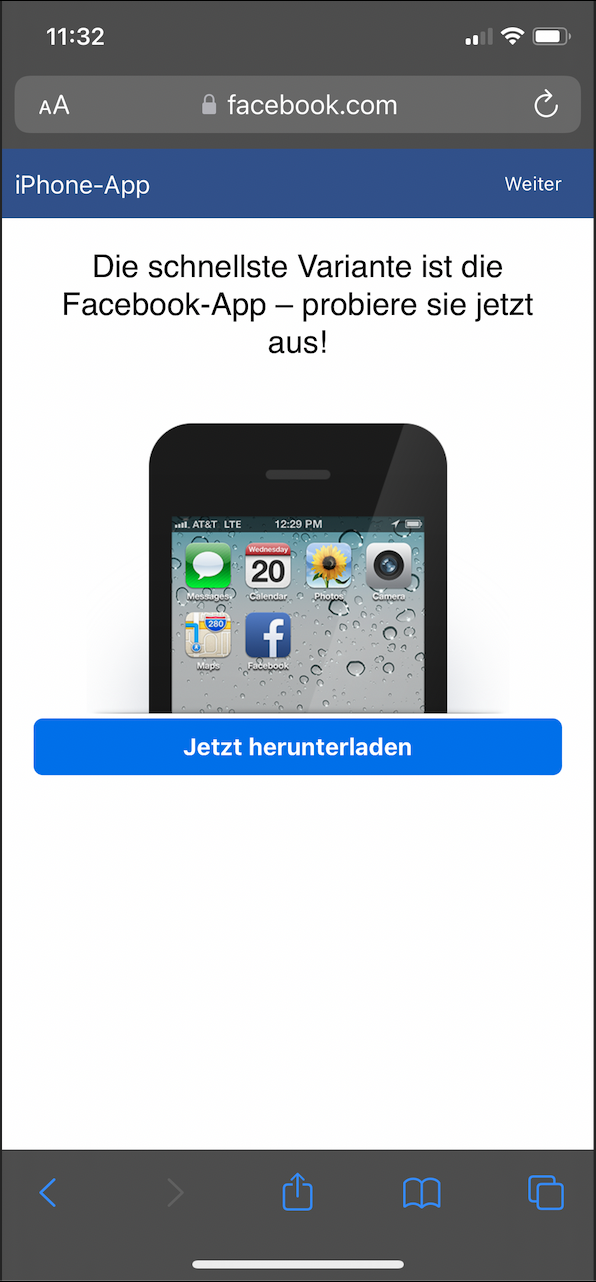
\includegraphics[scale=0.3]{_assets/facebook_native_app2.png} \\
	Facebook empfiehlt als einer der ersten Schritte nach der Registrierung via Smartphone-Webbrowser das Herunterladen der eigenen App.
\end{figure}

\end{document}



















